\chapter{Results}
\label{cha:results}

\section{From a User's Perspective}
\label{sec:results-user}

\begin{figure}
\centering
\begin{tabular}{ccc}
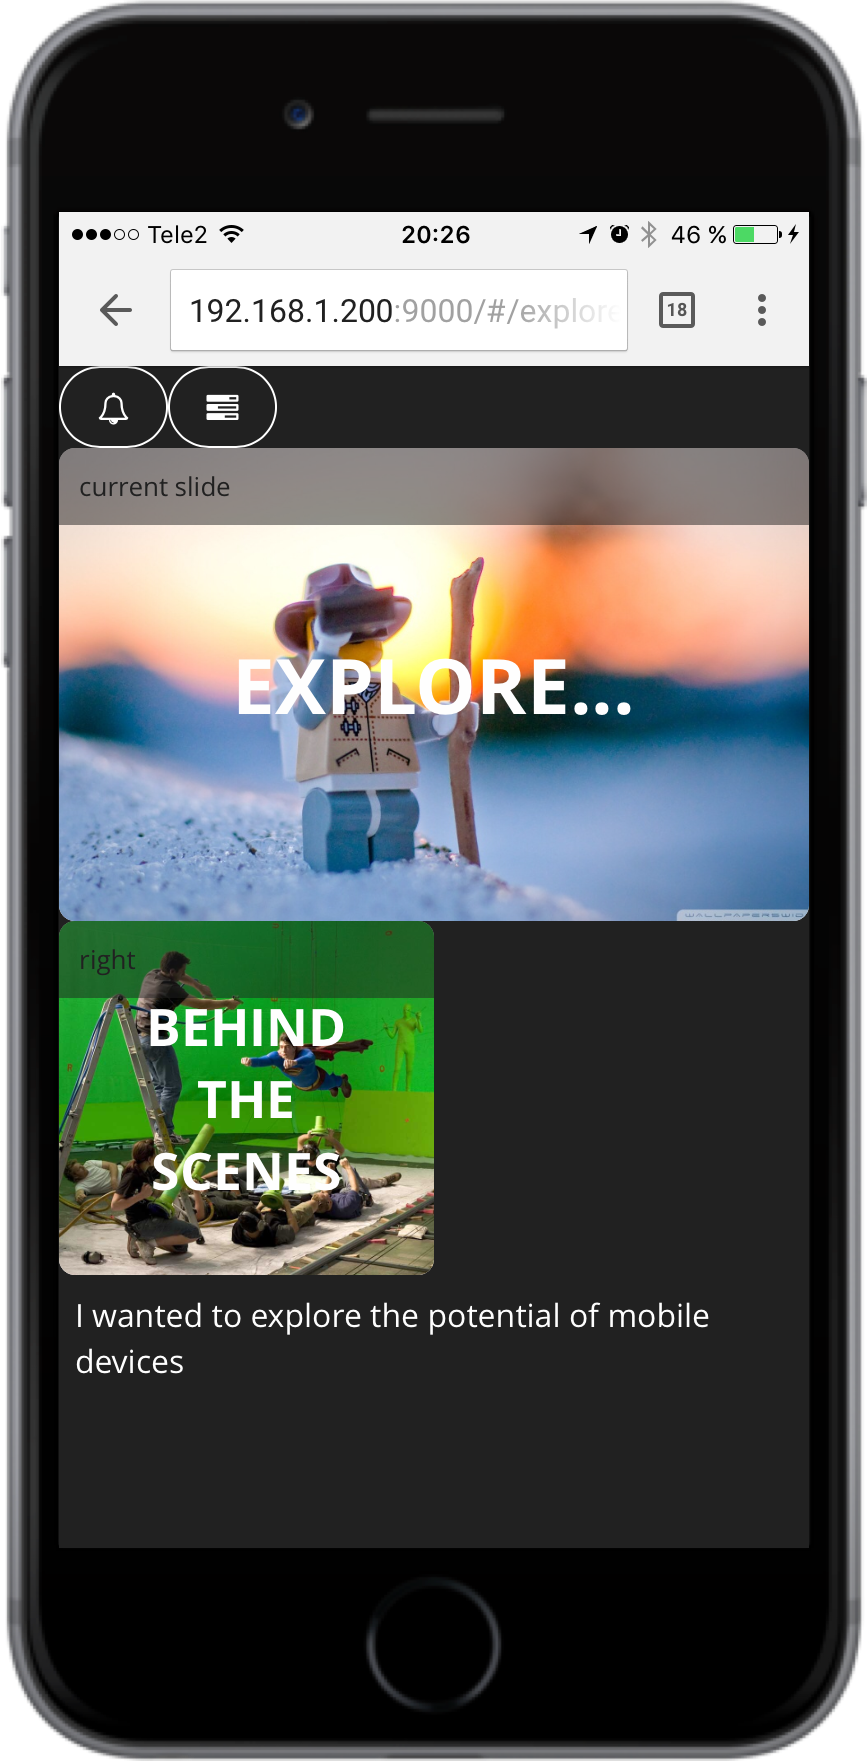
\includegraphics[width=.165\textwidth]{presenter-mode-mobile} &
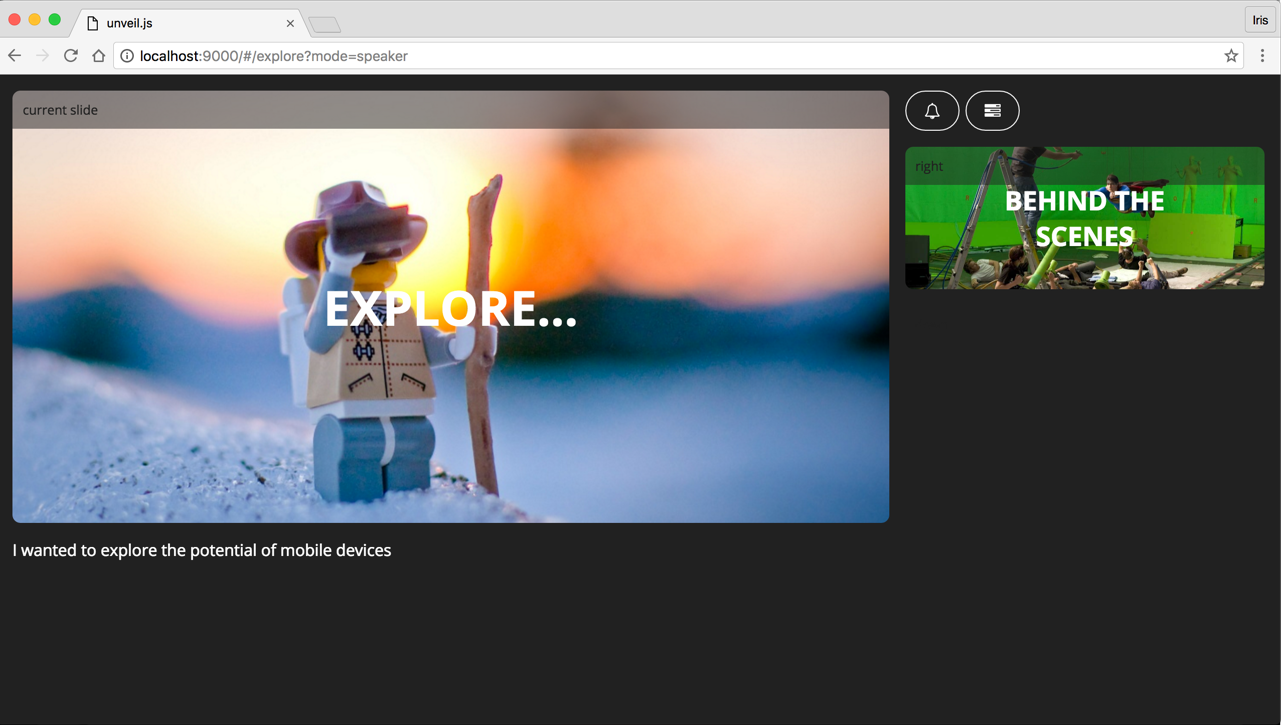
\includegraphics[width=.59\textwidth]{presenter-mode-desktop} \\
(a) & (b)
\end{tabular}
\caption{Speaker Presenter on mobile (a) and desktop (b).}
\label{fig:results-user-speaker-presenter}
\end{figure}

\begin{figure}
\centering
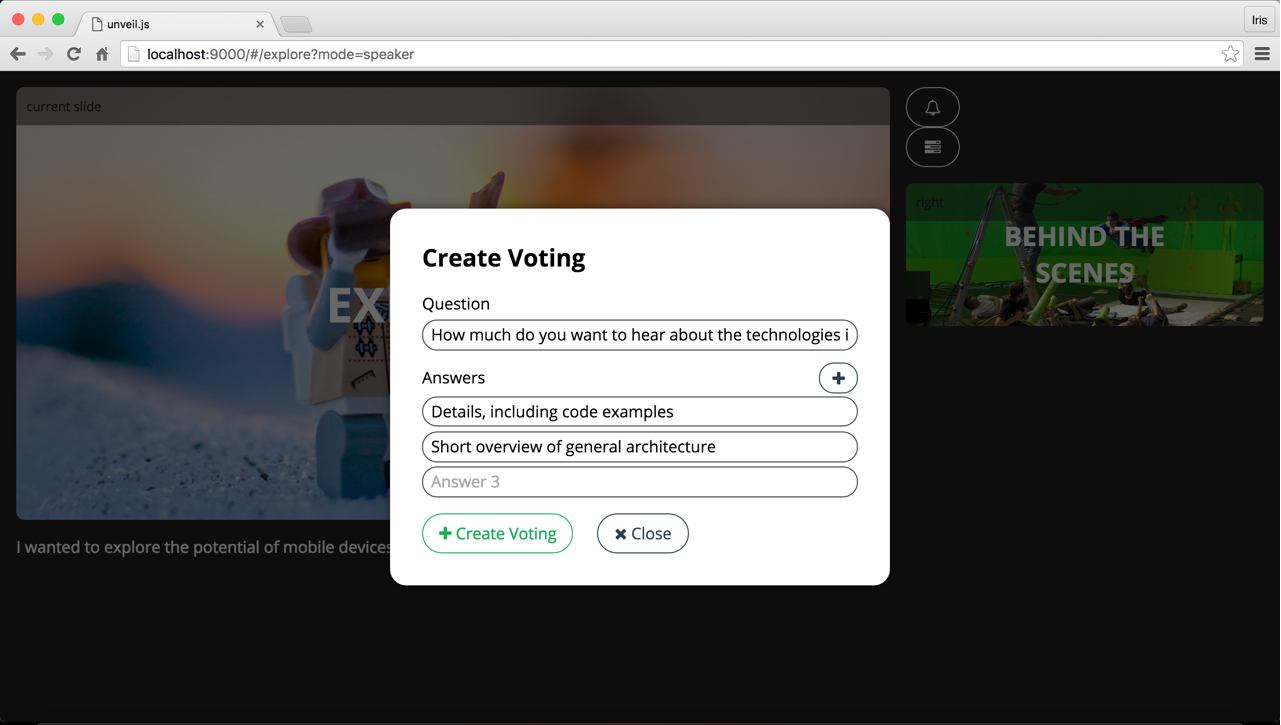
\includegraphics[width=.715\textwidth]{polls-modal}
\caption{Poll creation modal in presenter mode on tablets, laptops and desktops.}
\label{fig:results-user-polls-modal}
\end{figure}

\begin{figure}
\centering
\begin{tabular}{ccc}
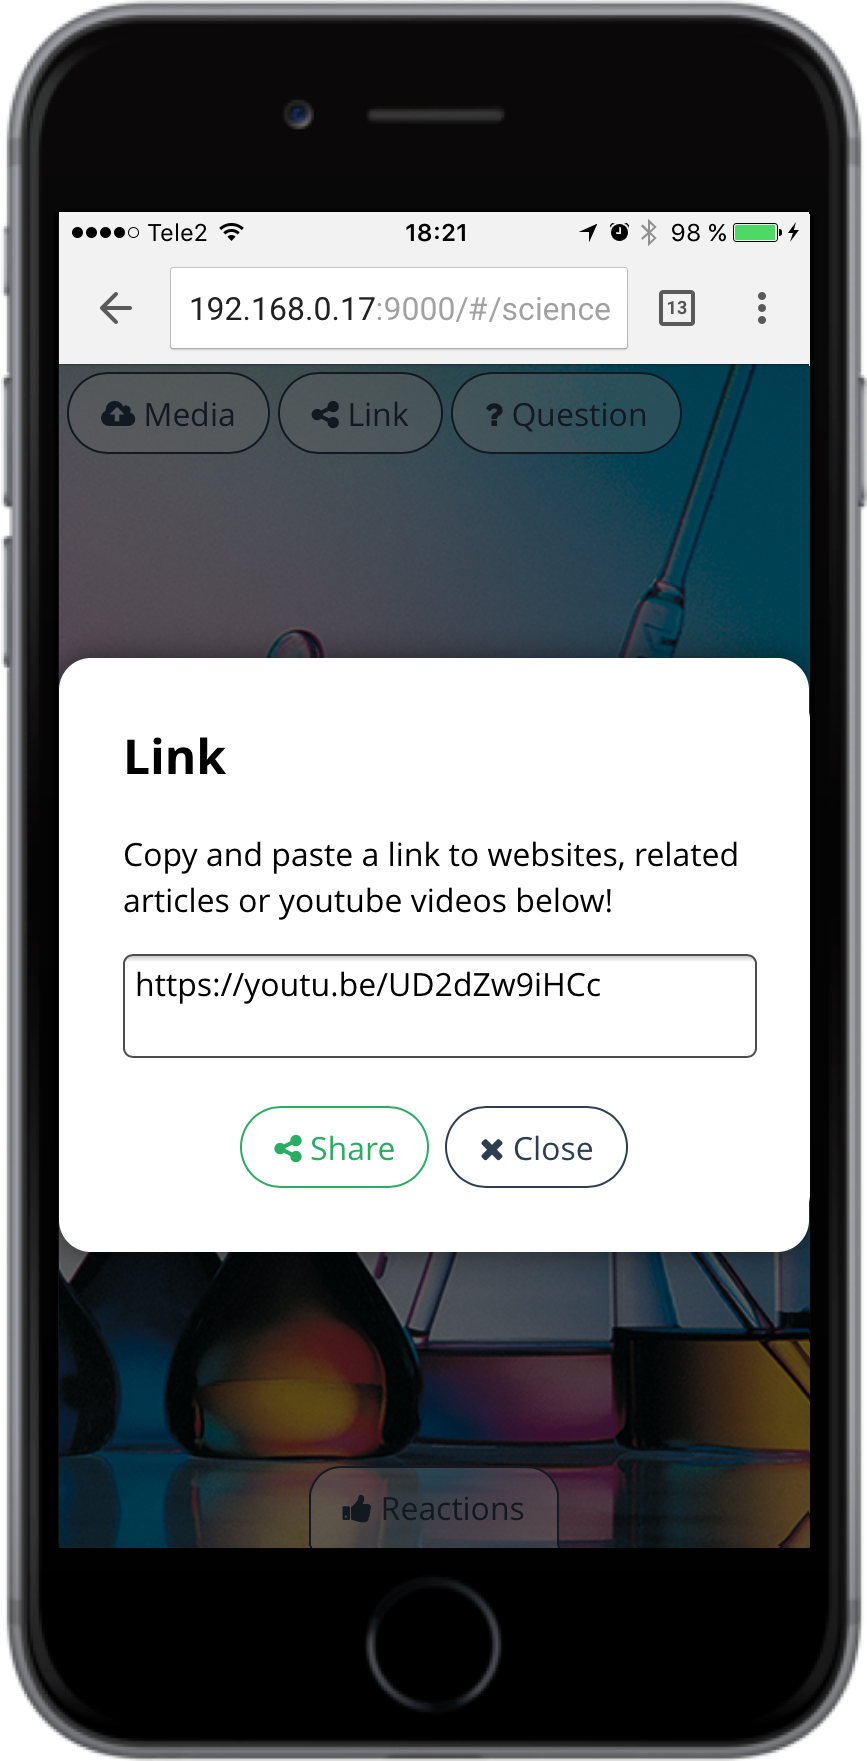
\includegraphics[width=.2\textwidth]{sharing-listener-youtube} &
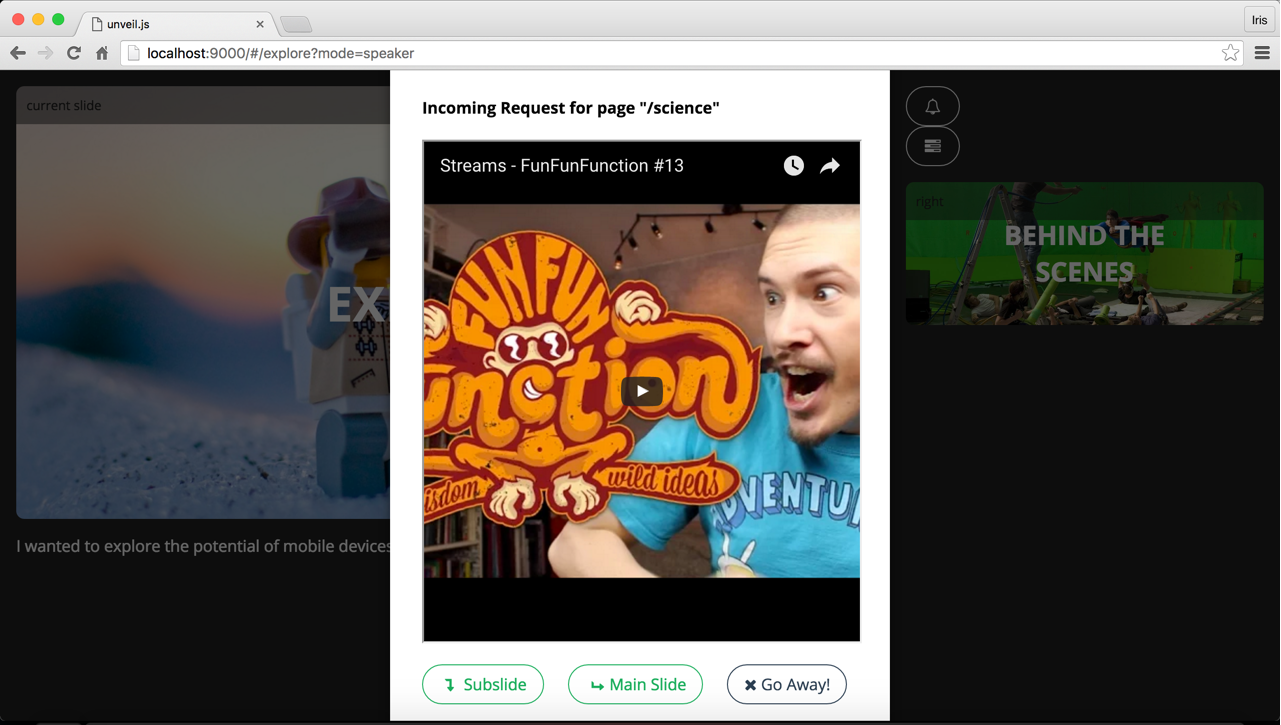
\includegraphics[width=.715\textwidth]{sharing-presenter-youtube} \\
(a) & (b)
\end{tabular}
\caption{Sharing of a youtube video. Request from listener on a phone (a) and accepting-modal in presenter-view on a computer (b).}
\label{fig:results-user-sharing-youtube}
\end{figure}

\begin{figure}
\centering
\begin{tabular}{ccc}
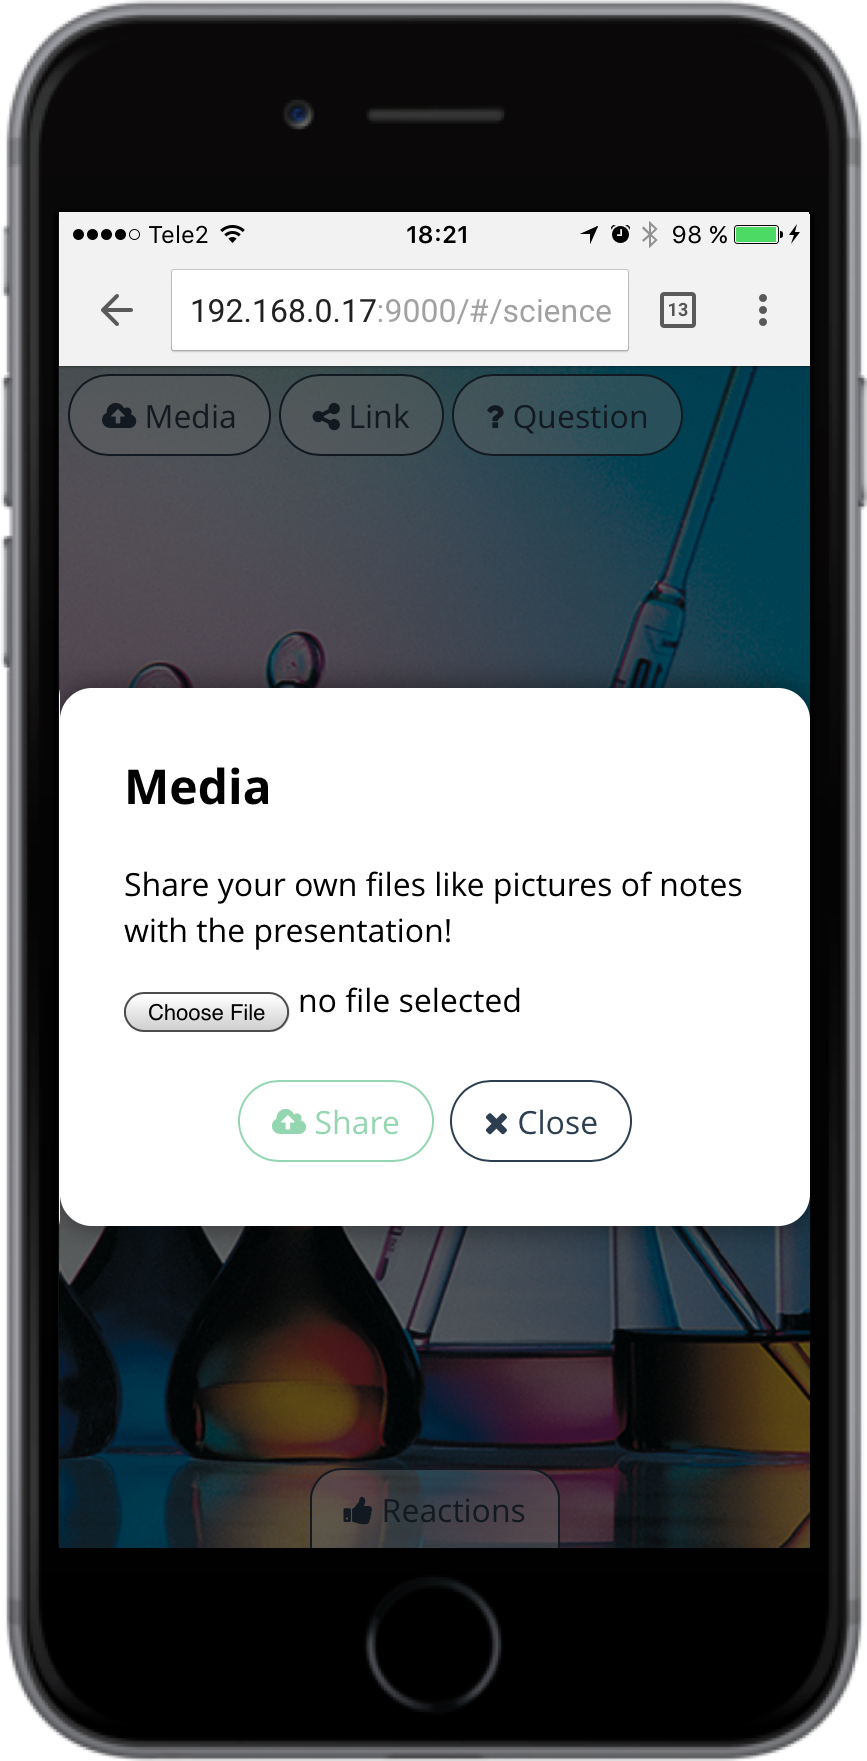
\includegraphics[width=.2\textwidth]{sharing-listener-1} &
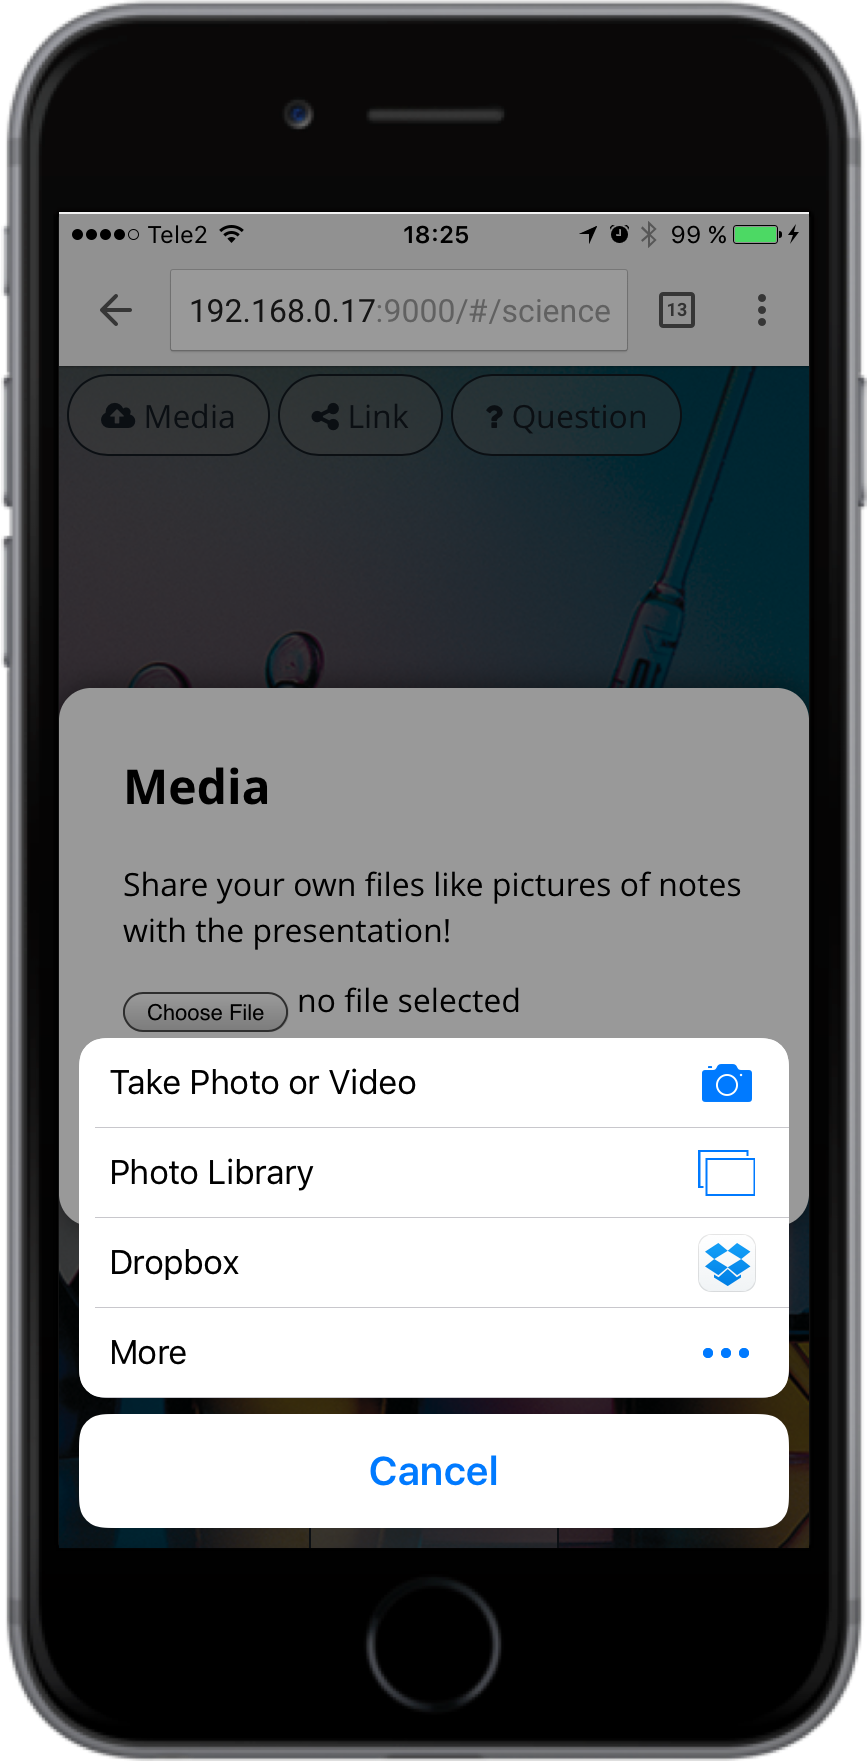
\includegraphics[width=.2\textwidth]{sharing-listener-2} &
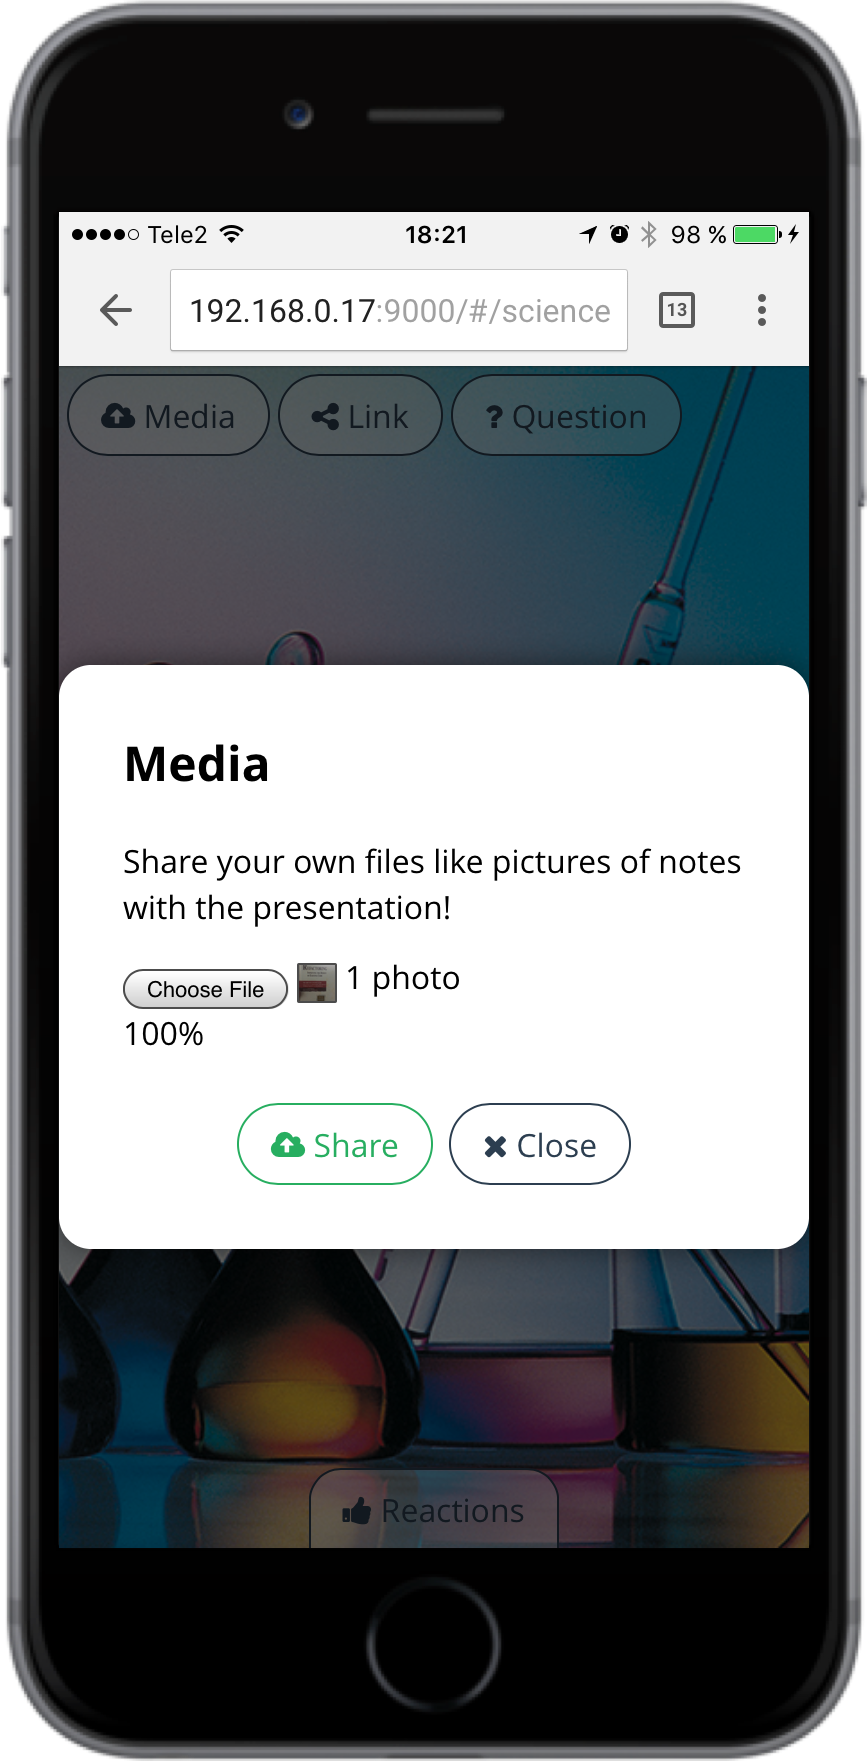
\includegraphics[width=.2\textwidth]{sharing-listener-3} \\
(a) & (b) & (c)
\end{tabular}
\caption{Sharing of a picture from an iPhone's browser (Google Chrome on iOS $9.3.4$) in listener mode. First, the listener opens the \emph{Media} sharing feature (a). Then a file can be chosen from different sources, such as the camera roll, or a new picture can be taken (b). In a last step, the picture is uploaded to the application and can then be shared (c).}
\label{fig:results-user-sharing-picture}
\end{figure}



\section{From a Developer's Perspective}
\label{sec:results-developer}

Since one of our declared goals was the creation of reusable, extensible presentation libraries, a few words should also be spent on the usage of the system by other developers. This chapter will therefore go into details of how to set up an unveil presentation (section \ref{sec:usage-setup}), use the components (section \ref{sec:usage-components}) and lastly ways of customising, overwriting and extending behaviour (section \ref{sec:usage-customisation}). The code-examples of this chapter are based on \cite{unveil-client-server}.

\section{Setup}
\label{sec:usage-setup}
% how is everything defined? what has to be included?
% what are the steps of building an application with unveil?
% how are the slides defined? how are they styled? what about the modes?

Since the entire created code is available on npm, the first step in setting up an unveil presentation is to require the necessary libraries \texttt{unveil}, \texttt{unveil-network-sync} and \texttt{unveil-interactive}. In the entry point of the presentation (usually \texttt{index.html}), all bundled JavaScript and CSS-files are included and an HTML document is created which offers a tag that can be used to render the presentation (e.g. a \texttt{div} with the class \texttt{unveil}). For lower the page loading time \cite{yahoo-speeding-up-website}, script tags should generally placed in the \texttt{body} tag, usually before closing said tag.
As soon as this initial page is set up, the actual presentation can be built in an JavaScript file which should also be included here.
In this file, we will call it \texttt{index.js} from now on, all necessary libraries and components are imported:  \texttt{React}, \texttt{ReactDom}, as well as all unveil components that should be used. If any libraries which rely on the communication with the WebSocket server should be used in the presentation, the \texttt{SocketIO} singelton also has to be configured with the address of the server:
\begin{GenericCode}
import { createSocket } from 'unveil-network-sync'
createSocket('http://192.168.0.17:9000')
\end{GenericCode}

\section{Building a Presentation}
\label{sec:usage-components}

Once all libraries are imported, the actual presentation can be created. The most important component in this context is \texttt{UnveilApp}, which is imported from \texttt{unveil}. This component holds all the \texttt{Slide}s and is responsible for the configuration of the application (see section \ref{sec:usage-customisation}). Inside the \texttt{Slide} components, all content of the slide and the \texttt{Notes} are placed. Each of the slides will be rendered as common HTML and can include any number of other HTML tags and custom React components (see programm \ref{prog:usage-presentation-creation}). Although strictly-speaking not necessary, it is recommended to give slides (unique) names, since their name will be the id of the rendered HTML component and makes it possible to style components with CSS (see programm \ref{prog:usage-styling}). Additionally, if provided, unveil uses the name of the current slide as the url, allowing for text-based rather than index-based routes.

Other than that, slides can have a \texttt{left}, \texttt{right}, \texttt{up} and \texttt{down} property to allow for several paths through a presentation: All slides are provided as normal slide-sets, but the \texttt{left} and \texttt{right} attributes of the first and last slide of each path point to the previous and next slide shared by the entire presentation. \texttt{Link}s (available in the \texttt{unveil-interactive} package) can be used to access the first slide of each path. Additionally, the interactive extension also offers the components for preparing votings: \texttt{Voting}, \texttt{Question} and \texttt{Answer} (see programm \ref{prog:usage-voting}). The only necessary property for \texttt{Voting}s is the \texttt{name} attribute, which uniquely identifies the voting, as well as exactly one \texttt{Question}-child and an arbitrary number of \texttt{Answer}s.

\begin{program}
\caption{Example styling unveil slides using Sass. In this particular piece of code, the font family of all slides is set and a background image is added to the slide of name \texttt{start}.}
\label{prog:usage-styling}
\begin{CssCode}
.slide
  font-family: 'Open Sans'
#start
  background-image: url('../img/explore.jpg')
\end{CssCode}
\end{program}

\begin{program}
\caption{Creation of a presentation. Sets up two slides as an example. The DOM will be attached to the element of id \texttt{unveil} in the base HTML document.}
\label{prog:usage-presentation-creation}
\begin{JsCode}
ReactDOM.render((
  <UnveilApp modes={modes}>
    <Slide name="start">
      <h1>Unveil</h1>
      <h2>a meta presentation</h2>
    </Slide>
    <Slide name="intro">
      <img src="./img/problem.png" />
      <Notes>Explain initial situation</Notes>
    </Slide>
    ...
  </UnveilApp>
), document.getElementById('unveil'))
\end{JsCode}
\end{program}


\begin{program}
\caption{Creation of votings in unveil. The necessary components have to be imported from \texttt{unveil-interactive}.}
\label{prog:usage-voting}
\begin{JsCode}
<Voting name="like">
  <Question>Do you like these slides?</Question>
  <Answer value="yes">Yes</Answer>
  <Answer value="no">No</Answer>
</Voting>
\end{JsCode}
\end{program}

\section{Customisation and Extension}
\label{sec:usage-customisation}

\begin{program}
\caption{Mode definition for setting up an unveil.js presentation. Default (i.e. listener) and speaker modes are omitted to keep the example short, but generally follow the same pattern as the projector mode.}
\label{fig:usage-modes}
\begin{JsCode}
const modes = {
  default: {...},
  speaker: {...},
  projector: {
    controls : [
      NavigationReceiver, MediaReceiver, ReactionReceiver,
      VotingNavigatableSetter, VotingReceiver
    ],
    presenter: Presenter
  }
};
\end{JsCode}
\end{program}

Thanks to unveil's base architecture, it is possible for speakers to entirely customise the entire presentation logic. The most important step is to define the available modes and the presenter and controls which should be loaded in each of them (see figure \ref{fig:usage-modes}). Additionally to the existing controls in unveil and its current extensions, new (presentation) logic can be added by defining ones own React components and assigning them to modes. To interact with the WebSocket server, \texttt{SocketIO} is available from the network synchronisation layer. Data such as the current router state or slide, and the navigator or state subject are accessible through \texttt{UnveilApp}'s context. For examples of existing controls and presenters, the reader is adviced to refer to the implementation of the components discussed in chapter \ref{cha:implementation} \cite{unveil-fork, unveil-network-sync, unveil-interactive}.

Moreover, the \texttt{Router} and \texttt{Navigator} can also be entirely replaced by providing ones own functionality as \texttt{router} and \texttt{navigator} properties in \texttt{UnveilApp}. They only have to follow the same interface as the default implementations. If any additional configuration should be necessary (such as with setting the address of the WebSocket server or customising emoji), singletons or static methods of the components can be used.
